\documentclass{article}
%% Useful packages
\usepackage[utf8]{inputenc}
\usepackage[a4paper,left=2cm,right=2cm,top=2cm,bottom=2cm]{geometry}
\usepackage{crop,graphicx,amsmath,array,color,amssymb,fancyhdr,lineno}
\usepackage{flushend,stfloats,amsthm,chngpage,times,,lipsum,lastpage} 
\usepackage{calc,listings,color,wrapfig,tabularx,longtable,enumitem}
\usepackage[style=numeric-comp,backend=biber]{biblatex}
\addbibresource{Refs.bib}
\usepackage{lineno}
%%%%%%%%%%%%   Header and Footer  %%%%%%%%%%%%%
\pagestyle{fancy}
\fancypagestyle{plain}{%
  \renewcommand{\headrulewidth}{0pt}%
  \fancyhf{}%
}

\title{%
  First Assignment \\
  \large Equivalent representations of orientation matrices}
\author{Surname Name}

\begin{document}
\begin{titlepage}

\newcommand{\HRule}{\rule{\linewidth}{0.5mm}} % Defines a new command for the horizontal lines, change thickness here

%----------------------------------------------------------------------------------------
%	LOGO SECTION
%----------------------------------------------------------------------------------------
\center

\includegraphics[width=5cm]{Title/Unige-logo.jpeg}\\[1cm] % Include a department/university logo - this will require the graphicx package
 
%----------------------------------------------------------------------------------------

\center % Center everything on the page

%----------------------------------------------------------------------------------------
%	HEADING SECTIONS
%----------------------------------------------------------------------------------------

\textsc{\Huge Università degli studi di Genova}\\[1cm] % Name of your university/college
\textsc{\LARGE DIBRIS}\\[0.3cm]
\textsc{\Small Department of Computer Science and Technology,}\\
\textsc{\Small Bioengineering, Robotics and System Engineering}\\[1cm] % Minor heading such as course title
\textsc{\LARGE{Modelling and Control of Manipulators}}\\[1cm] % Major heading such as course name

%----------------------------------------------------------------------------------------
%	TITLE SECTION
%----------------------------------------------------------------------------------------
\makeatletter
\HRule \\[0.4cm]
{ \huge \bfseries First Assignment}\\[0.2cm] 
{\Large \bfseries Equivalent representations of orientation matrices}\\
% Title of your document
\HRule \\[1.5cm]
 
%----------------------------------------------------------------------------------------
%	AUTHOR SECTION
%----------------------------------------------------------------------------------------

\begin{minipage}{0.4\textwidth}
\begin{flushleft} \large
\emph{Author:}\\[0.2cm]
Khadka Chhetri Rubin % Your name
\\[1.2em]
\emph{Student ID:}\\[0.2cm]
s6558048 \\[1.2em]
\end{flushleft}
\end{minipage}
~
\begin{minipage}{0.4\textwidth}
\begin{flushright} \large
\emph{Professors:} \\[0.2cm]
Giovanni Indiveri\\
Enrico Simetti\\
Giorgio Cannata  \\[1.2em] % Supervisor's Name

\emph{Tutors:} \\[0.2cm]
Andrea Tiranti\\
Georgii Kurshakov\\
Luca Tarasi
% second marker's name
\end{flushright}
\end{minipage}\\[2cm]
\makeatother

% If you don't want a supervisor, uncomment the two lines below and remove the section above
%\Large \emph{Author:}\\
%John \textsc{Smith}\\[3cm] % Your name

%----------------------------------------------------------------------------------------
%	DATE SECTION
%----------------------------------------------------------------------------------------

{\large \today}\\[2cm] % Date, change the \today to a set date if you want to be precise

\vfill % Fill the rest of the page with whitespace

\end{titlepage}

\sffamily

\fancyhf{}
\fancyhead[L]{Khadka Chhetri Rubin - s6558048}
\fancyhead[R]{Modelling and Control of Manipulators - Assignment 1}
\fancyfoot[R]{ \bf\thepage\ \rm }%

\newpage
\tableofcontents

\section*{}
\begin{longtable}{|p{4cm}|p{4cm}|p{4cm}|}
    \hline
    Mathematical expression & Definition & MATLAB expression \\
    \hline 
    $<w>$ & World Coordinate Frame &  w\\[0.4cm]
    $^a_b R$ & Rotation matrix of frame $<b>$ with respect to frame $<a>$  & aRb \\[1.2cm]
    $^a_b T$ & Transformation matrix of frame $<b>$ with respect to frame $<a>$ & aTb \\[1.2cm]
    \hline
    \caption{Nomenclature Table}
\end{longtable}

\section{Assignment description}
The first assignment of Modelling and Control of Manipulators focuses on the geometric fundamentals and algorithmic tools underlying any robotics application. The concepts of transformation matrix, orientation matrix and the equivalent representations of orientation matrices (Equivalent angle-axis representation and Euler Angles) will be reviewed.

The first assignment is \textbf{mandatory} and consists of 5 different exercises. You are asked to:
\begin{itemize}
    \item Download the .zip file called MCM-LAB1 from the Aulaweb page of this course.
    \item Implement the code to solve the exercises on MATLAB by filling the predefined files called "\textit{main.m}", "\textit{AngleAxisToRot.m}", "\textit{RotToAngleAxis.m}", "\textit{YPRToRot.m}" and "\textit{RotToYPR.m}".
    \item Write a report motivating the answers for each exercise, following the predefind format on this document.
\end{itemize}

\subsection{Exercise 1 - Angle-Axis to Rotation Matrix}
A particularly interesting minimal representation of 3D rotation matrices is the so-called angle-axis representation, where a rotation is represent by the axis of rotation \begin{math}\textbf{h}\end{math} and the angle $\theta$. Any rotation matrix can be represented by its equivalent angle-axis representation by applying the Rodrigues Formula.

%\[ R(^* \textbf{v},\theta) = e^{[^*\textbf{v}\times]\theta} = e^{[\rho\times]} =  \textbf{I}_{3x3} + [^* \textbf{v}\times] \sin(\theta) + [^* \textbf{v}\times]^2 (1-\cos(\theta))\]


\textbf{Q1.1} Given an angle-axis pair \begin{math}(\textbf{h},\theta)\end{math}, implement on MATLAB the Rodrigues formula, computing the equivalent rotation matrix, \textbf{WITHOUT} using built-in matlab functions. The function signature will be


\begin{center}\textit{function R = AngleAxisToRot(h,theta)}\end{center}


Then test it for the following cases and briefly comment the results obtained:
\begin{itemize}
    \item \textbf{Q1.2}\hspace{10mm} \begin{math} \textbf{h} = [1,0,0]^T\end{math} and  \begin{math} \theta = 90^\circ \end{math}
    \item \textbf{Q1.3}\hspace{10mm} \begin{math} \textbf{h} = [0,0,1]^T\end{math} and  \begin{math} \theta = \pi/3 \end{math}
    \item \textbf{Q1.4}\hspace{10mm} \begin{math} \mathbf{\rho} = [-\pi/3, -\pi/6 ,\pi/3];\end{math}
\end{itemize}
\textbf{Note that $\mathbf{\rho} = \textbf{h}\theta$}.
%\subsection{Exercise 2 - Inverse Equivalent Angle-Axis Problem}
\subsection{Exercise 2 - Rotation Matrix to Angle-Axis}
Given a rotation matrix \begin{math}R\end{math}, the problem of finding the corresponding angle-axis representation \begin{math}(\textbf{h},\theta)\end{math} is called the Inverse Equivalent Angle-Axis Problem.
\newline


\textbf{Q2.1} Given a rotation matrix \begin{math}R\end{math}, implement on MATLAB the Equivalent Angle-Axis equations \textbf{WITHOUT} using built-in matlab functions. The function signature will be


\begin{center}\textit{function [h,theta] = RotToAngleAxis(R)}\end{center}


You \textbf{MUST} check that the input is a valid rotation matrix. Test it for the following cases and briefly comment the results obtained:

\begin{itemize}
    \item \textbf{Q2.2}\hspace{10mm} $R = \begin{pmatrix}
        1 & 0 & 0 \\
        0 & 0 & -1 \\
        0 & 1 & 0
    \end{pmatrix}$
    
    \item \textbf{Q2.3}\hspace{10mm} $R = \begin{pmatrix}
        0.5& -\sqrt{3}/2 & 0 \\
        \sqrt{3}/2 & 0.5 & 0 \\
        0 & 0 & 1
    \end{pmatrix}$
    
    \item \textbf{Q2.4}\hspace{10mm} $R = \begin{pmatrix}
        1 & 0 & 0 \\
        0 & 1 & 0 \\
        0 & 0 & 1
    \end{pmatrix}$
    
    \item \textbf{Q2.5}\hspace{10mm} $R = \begin{pmatrix}
        -1 & 0 & 0 \\
        0 & -1 & 0 \\
        0 & 0 & 1
    \end{pmatrix}$
\end{itemize}

\subsection{Exercise 3 - Euler Angles to Rotation Matrix}
Any orientation matrix can be expressed in terms of three elementary rotations in sequence. Consider the Yaw Pitch Roll (YPR) representation, where the sequence of the rotation axes is Z-Y-X.
\newline

\textbf{Q3.1} Given a triplet of YPR angles ($\psi$, $\theta$, $\phi$), compute the equivalent rotation matrix representation \textbf{WITHOUT} using built-in matlab functions. The function signature will be


\begin{center}\textit{function R = YPRToRot(psi, theta, phi)}\end{center}


Then test it for the following cases and briefly comment the results obtained:


\begin{itemize}
    \item \textbf{Q3.2}\hspace{10mm} $\psi=\theta=0$, $\phi=\pi/2$
    \item \textbf{Q3.3}\hspace{10mm} $\phi=\theta=0$, $\psi=60^\circ$
    \item \textbf{Q3.4}\hspace{10mm} $\psi=\pi/3$, $\theta=\pi/2$, $\phi=\pi/4$
    \item \textbf{Q3.5}\hspace{10mm} $\psi=0$, $\theta=\pi/2$, $\phi=-\pi/12$
\end{itemize}

\subsection{Exercise 4 - Rotation Matrix to Euler Angles}
Given a rotation matrix \begin{math}R\end{math}, it is possible to compute an equivalent triplet of YPR angles ($\psi$, $\theta$, $\phi$), provided that the configuration is not singular (that is, $\cos{\theta} \ne 0$).
\newline

\textbf{Q4.1} Given a rotation matrix \begin{math}R\end{math}, implement in MATLAB the equivalent YPR angles, \textbf{WITHOUT} using built-in matlab functions. The function signature will be


\begin{center}\textit{function [psi,theta,phi] = rotToYPR(R)}\end{center}


You \textbf{MUST} check that the input is a valid rotation matrix. Test it for the following cases and briefly comment the results obtained:


\begin{itemize}
    \item $\textbf{Q4.2}\hspace{10mm} R = \begin{pmatrix}
        1 & 0 & 0 \\
        0 & 0 & -1 \\
        0 & 1 & 0
    \end{pmatrix}$
    
    \item $\textbf{Q4.3}\hspace{10mm} R = \begin{pmatrix}
        \frac{1}{2} & -\frac{\sqrt{3}}{2} & 0 \\
        \frac{\sqrt{3}}{2} & \frac{1}{2} & 0 \\
        0 & 0 & 1
    \end{pmatrix}$
    
    \item $\textbf{Q4.4}\hspace{10mm} R = \begin{pmatrix}
        0 & -\frac{\sqrt{2}}{2} & \frac{\sqrt{2}}{2} \\
        0.5 & \frac{\sqrt{2}\sqrt{3}}{4} & \frac{\sqrt{2}\sqrt{3}}{4} \\
        -\frac{\sqrt{3}}{2} & \frac{\sqrt{2}}{4} & \frac{\sqrt{2}}{4}
    \end{pmatrix}$
\end{itemize}

\subsection{Exercise 5 - Frame tree}

\begin{figure}
\centering
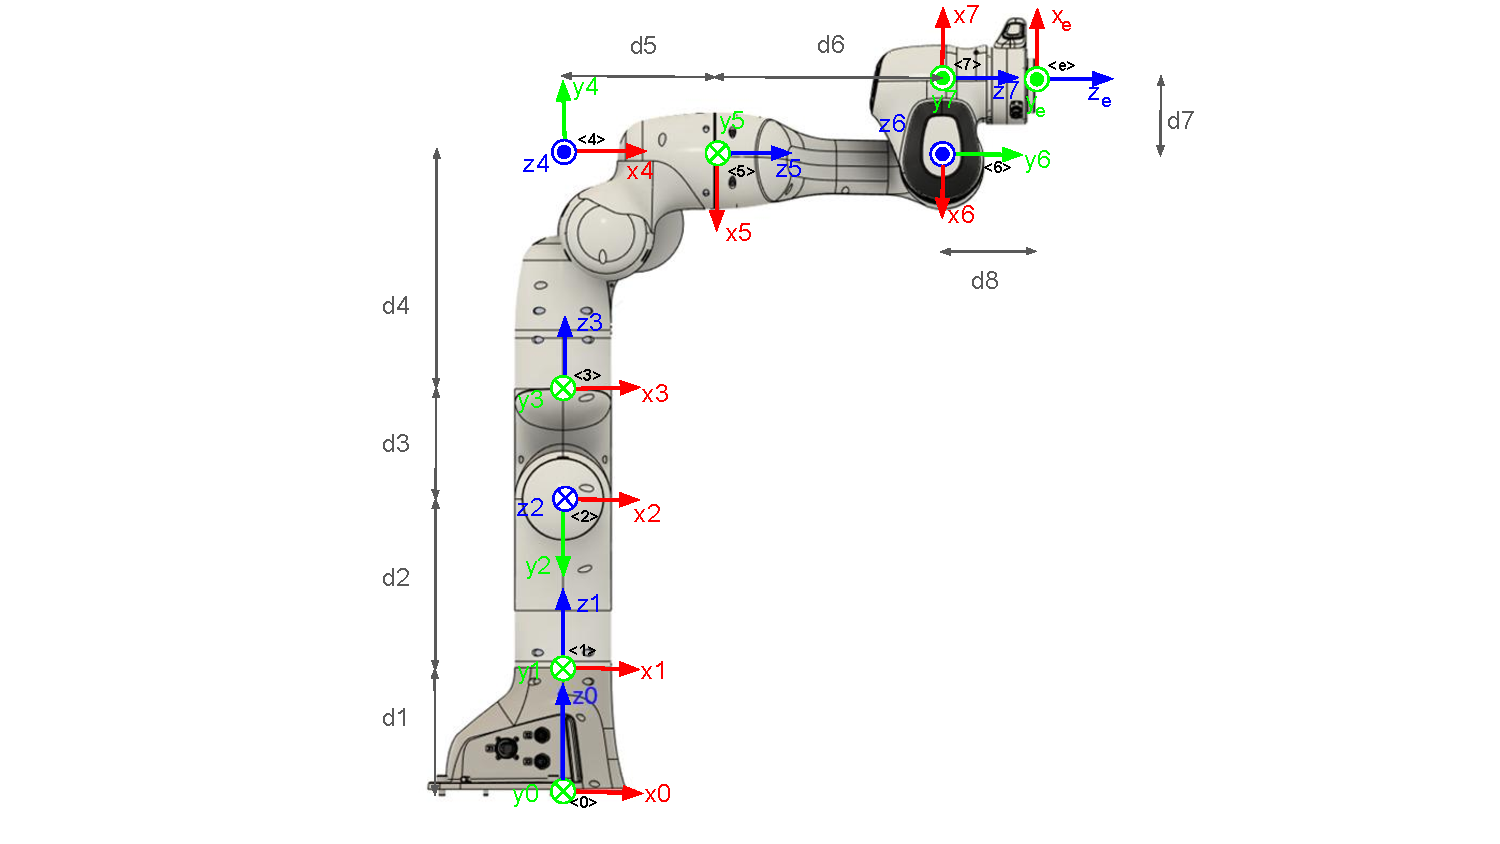
\includegraphics[width=1\linewidth]{Resources/franka.pdf}
\caption{exercise 5 frames}
\label{fig:ex2}
\end{figure}

Figure \ref{fig:ex2} shows the frame tree for the 7 joints of the Franka robot. With reference to the figure, use the geometric definition of the transformation matrix to compute by hand the following matrices.
\begin{itemize}
\item \textbf{Q5.1} \hspace{10mm} $^0_1 T$
\item \textbf{Q5.2} \hspace{10mm} $^1_2 T$
\item \textbf{Q5.3} \hspace{10mm} $^2_3 T$
\item \textbf{Q5.4} \hspace{10mm} $^3_4 T$
\item \textbf{Q5.5} \hspace{10mm} $^4_5 T$
\item \textbf{Q5.6} \hspace{10mm} $^5_6 T$
\item \textbf{Q5.7} \hspace{10mm} $^6_7 T$
\item \textbf{Q5.8} \hspace{10mm} $^7_e T$
\end{itemize}

You \textbf{MUST} compute the matrices \textbf{WITHOUT} using mathematical software.

\newpage

\section{Exercise 1 - Angle-Axis to Rotation Matrix} \label{P1}
In this exercise, the conversion from angle-axis representation to a rotation matrix is implemented using the Rodrigues formula, expressed as:

\begin{equation} \label{rodrigues_formula}
R(\mathbf{h}, \theta) = I_{3 \times 3} + [\mathbf{K}] \sin \theta + [\mathbf{K}]^2 (1 - \cos \theta)
\end{equation}

In this formula, \( R \) represents the rotation matrix, \( I_{3 \times 3} \) is the identity matrix, \( \theta \) denotes the angle of rotation, and \( [\mathbf{K}] \) is the skew-symmetric matrix derived from the axis of rotation \( \mathbf{h} \). This method allows the representation of a rotation in three-dimensional space using a given axis of rotation and angle.

\subsection{Q 1.1 - Implementation of Angle-Axis to Rotation Matrix Conversion}

A MATLAB function \texttt{AngleAxisToRot} was implemented to convert an angle-axis representation into a rotation matrix using the Rodrigues formula. The function accepts two inputs: the axis of rotation \( \mathbf{h} \) and the angle of rotation \( \theta \) in radians. The following steps are followed in the function:

\begin{enumerate}
    \item \textbf{Normalization of the Axis Vector:}
    The input axis vector \( \mathbf{h} \) is normalized to ensure it has a unit length. This normalization is crucial because it preserves the direction of the axis while setting its magnitude to 1.

    \item \textbf{Skew-Symmetric Matrix Construction:}
    A skew-symmetric matrix \( [\mathbf{K}] \) is then constructed from the components of the normalized axis vector. This matrix is used in the Rodrigues formula to compute the rotation matrix:
    \begin{equation}
    [\mathbf{K}] = \begin{bmatrix}
    0 & -h_3 & h_2 \\
    h_3 & 0 & -h_1 \\
    -h_2 & h_1 & 0
    \end{bmatrix}
    \end{equation}
    
    \item \textbf{Identity Matrix:}
    The identity matrix \( I_{3 \times 3} \) (a 3x3 identity matrix) is created using the \texttt{eye(3)} function to serve as the foundation for the rotation matrix calculation.
    
    \item \textbf{Rotation Matrix Calculation:}  
    Finally, the rotation matrix \( R \) is computed using the Rodrigues formula (Equation~\ref{rodrigues_formula}). This combines the identity matrix, the skew-symmetric matrix multiplied by the sine of the rotation angle, and the skew-symmetric matrix squared multiplied by \( (1 - \cos(\theta)) \). In MATLAB, this calculation is executed as:
    \begin{verbatim}
    R = I + sin(theta) * K + (1 - cos(theta)) * (K * K);
    \end{verbatim}
\end{enumerate}
The complete function code can be found in Appendix A.

\subsection{Q 1.2 -  Test Case 1}
For the test case with axis \( \mathbf{h} = [1, 0, 0]^T \) and angle \( \theta = 90^\circ \) (or \( \theta = \frac{\pi}{2} \) radians), the rotation matrix obtained is as follows:

\[
R = \begin{bmatrix}
1.0000 & 0 & 0 \\
0 & 0.0000 & -1.0000 \\
0 & 1.0000 & 0.0000
\end{bmatrix}
\]

\begin{itemize}
    \item The first row \([1.0000, 0, 0]\) confirms that the x-coordinate remains unchanged after the rotation.
    \item The second row \([0, 0.0000, -1.0000]\) shows that the original y-axis rotates downward to align with the negative z-axis.
    \item The third row \([0, 1.0000, 0.0000]\) indicates that the original z-axis moves upward to align with the positive y-axis.
\end{itemize}

This result demonstrates that points initially in the yz-plane are now positioned in the xz-plane with a 90-degree rotation about the x-axis.

\subsection{Q 1.3 -  Test Case 2}
For the test case with axis \( \mathbf{h} = [0, 0, 1]^T \) and angle \( \theta = \frac{\pi}{3} \) radians, the rotation matrix obtained is as follows:

\[
R = \begin{bmatrix}
0.5000 & -0.8660 & 0 \\
0.8660 & 0.5000 & 0 \\
0 & 0 & 1.0000
\end{bmatrix}
\]

\begin{itemize}
    \item The third row \([0, 0, 1.0000]\) shows that the z-coordinate remains unchanged.
    \item The first row \([0.5000, -0.8660, 0]\) shows that a point originally located on the x-axis now lies in the xy-plane, positioned at an angle of \( 60^\circ \) from the x-axis.
    \item The second row \([0.8660, 0.5000, 0]\) indicates that a point initially on the y-axis rotates to align with the positive x-axis.
\end{itemize}

Thus, points initially in the xy-plane are now at a \( 60^\circ \) angle relative to the x-axis with the rotation about the z-axis.

\subsection{Q 1.4 -  Test Case 3}
For the test case with \(\rho = [-\frac{\pi}{3}, -\frac{\pi}{6}, \frac{\pi}{3}]\), the rotation matrix obtained is:

\[
R = \begin{bmatrix}
0.4444 & -0.4444 & -0.7778 \\
0.8889 & 0.1111 & 0.4444 \\
-0.1111 & -0.8889 & 0.4444
\end{bmatrix}
\]

In this case, the angle \(\theta\) and axis \(h\) were computed from \(\rho\) as follows:
\begin{equation}
\mathbf{h} = \frac{\rho}{\|\rho\|}, \quad \theta = \|\rho\|
\end{equation}

Here, \( \|\rho\| \) is the norm of \( \rho \).

\begin{itemize}
    \item The first row \([0.4444, -0.4444, -0.7778]\) shows how points originally along the x-axis are transformed, indicating a rotation influenced by both the x and y axes.
    \item The second row \([0.8889, 0.1111, 0.4444]\) suggests that points initially aligned with the y-axis are rotated, primarily influenced by the positive x and z components.
    \item The third row \([-0.1111, -0.8889, 0.4444]\) reveals how points on the z-axis are affected, indicating a rotation that pushes them towards the negative x-direction while being influenced positively along the y-direction.
\end{itemize}


\section{Exercise 2 - Rotation Matrix to Angle-Axis} \label{P2}

In this exercise, the conversion from a rotation matrix to its equivalent angle-axis representation is implemented. Given a rotation matrix \( R \), the angle of rotation \( \theta \) and the corresponding axis of rotation \( \mathbf{h} \) are determined.

The angle-axis representation is derived from the rotation matrix using the following relationships:

\begin{equation} \label{angle_axis}
\theta = \cos^{-1} \left( \frac{\text{tr}(R) - 1}{2} \right)
\end{equation}

where \( \text{tr}(R) \) denotes the trace of the matrix \( R \). The axis of rotation \( \mathbf{h} \) is calculated using:

\begin{equation} \label{axis}
\mathbf{h} = \frac{1}{\sqrt{1 + R_{11} + R_{22} + R_{33}}} \begin{bmatrix}
R_{32} - R_{23} \\
R_{13} - R_{31} \\
R_{21} - R_{12}
\end{bmatrix}
\end{equation}

This method enables the orientation of a rotation to be expressed as a vector and an angle.

\subsection{Q 2.1 - Implementation of Rotation Matrix to Angle-Axis Conversion}

A MATLAB function, \texttt{RotToAngleAxis}, was implemented to convert a rotation matrix \( R \) into its angle-axis representation \( (\mathbf{h}, \theta) \). The function operates as follows:

\begin{enumerate}
    \item \textbf{Validation of Rotation Matrix:}
    The input rotation matrix \( R \) is first verified as a valid rotation matrix through several checks:
    \begin{itemize}
        \item \textit{Size Check:} The dimensions of the matrix are confirmed to be \( 3 \times 3 \) by verifying both dimensions equal 3. If this condition is not met, an error is raised.
        
        \item \textit{Orthogonality Check:} The orthogonality of \( R \) is checked by computing the product \( R R^T \) and comparing it to the identity matrix \( I \). This step ensures that the rows (and columns) of \( R \) are orthonormal vectors.
        
        \item \textit{Determinant Check:} The determinant of the matrix is calculated, and it is verified to equal 1.
    \end{itemize}

    \item \textbf{Angle of Rotation:}
    The angle \( \theta \) of rotation is then calculated from the trace of the rotation matrix using Equation~\ref{angle_axis}. This angle represents the amount of rotation about the axis \( \mathbf{h} \).

    \item \textbf{Axis Vector Calculation:}
    The axis of rotation \( \mathbf{h} \) is calculated from a skew-symmetric matrix \( \mathbf{K} \), derived from the rotation matrix \( R \). The skew-symmetric matrix is calculated using the following formula:
    \begin{equation} \label{skew_symmetric}
    \mathbf{K} = \frac{R - R^T}{2 \sin(\theta)}
    \end{equation}
    The corresponding vector is then extracted using the \texttt{vex} function, which converts the skew-symmetric matrix \( \mathbf{K} \) into a vector that represents the rotation axis. Specifically, the components from the matrix are extracted as follows:
    
    \begin{equation}
    \mathbf{h} = \begin{bmatrix}
    K_{32} \\
    K_{13} \\
    K_{21}
    \end{bmatrix}
    \end{equation}
    
    where \( K_{ij} \) denotes the element in the \( i \)-th row and \( j \)-th column of the matrix \( \mathbf{K} \). This results in a standard 3D vector format that represents the rotation axis.
    
    The axis vector \( \mathbf{h} \) is normalized to ensure it is a unit vector:
    
    \begin{equation}
    \mathbf{h} = \frac{\mathbf{h}}{\|\mathbf{h}\|}
    \end{equation}
    
    where \( \|\mathbf{h}\| \) represents the norm (magnitude) of the vector \( \mathbf{h} \).

    \item \textbf{Output:}
    Finally, the calculated axis vector \( \mathbf{h} \) and the angle \( \theta \) in radians are returned.
\end{enumerate}

\subsection{Q 2.2 - Test Case 1}
The rotation matrix used in Test Case 1 is:
\[
R = 
\begin{bmatrix}
1 & 0 & 0 \\
0 & 0 & -1 \\
0 & 1 & 0
\end{bmatrix}
\]

The output obtained from Test Case 1 is as follows:
\begin{align*}
\text{Rotation axis } (\mathbf{h}) &= 
\begin{bmatrix}
1 \\
0 \\
0
\end{bmatrix} \\
\text{Angle } (\theta) &= 1.5708 \text{ radians (or } 90^\circ\text{)}
\end{align*}

These results indicate that the rotation axis is aligned with the x-axis, and the angle of rotation is \( 90^\circ \). It is confirmed that the rotation represented by the matrix \( R \) corresponds to a \( 90^\circ \) rotation about the x-axis, which aligns with the properties of the given matrix.

\subsection{Q 2.3 - Test Case 2}

The rotation matrix used in Test Case 2 is:
\[
R = 
\begin{bmatrix}
0.5 & -\frac{\sqrt{3}}{2} & 0 \\
\frac{\sqrt{3}}{2} & 0.5 & 0 \\
0 & 0 & 1
\end{bmatrix}
\]

The output obtained from Test Case 2 is as follows:
\begin{align*}
\text{Rotation axis } (\mathbf{h}) &= 
\begin{bmatrix}
0 \\
0 \\
1
\end{bmatrix} \\
\text{Angle } (\theta) &= 1.0472 \text{ radians (or } 60^\circ\text{)}
\end{align*}

These results indicate that the rotation axis is aligned with the z-axis, and the angle of rotation is \( 60^\circ \). It is confirmed that the rotation represented by the matrix \( R \) corresponds to a \( 60^\circ \) rotation about the z-axis, which aligns with the properties of the given matrix.

\subsection{Q 2.4 - Test Case 3}

The rotation matrix used in Test Case 3 is:
\[
R = 
\begin{bmatrix}
1 & 0 & 0 \\
0 & 1 & 0 \\
0 & 0 & 1
\end{bmatrix}
\]

The output obtained from Test Case 3 is as follows:
\begin{align*}
\text{Rotation axis } (\mathbf{h}) &= 
\begin{bmatrix}
0 \\
0 \\
0
\end{bmatrix} \\
\text{Angle } (\theta) &= 0 \text{ radians}
\end{align*}

These results show that the rotation axis is undefined because the input matrix represents the identity transformation, which corresponds to no rotation. The angle of rotation being \( 0 \) confirms that there is no change in orientation, consistent with the properties of the identity matrix.

\subsection{Q 2.5 - Test Case 4}
The rotation matrix used in Test Case 4 is:
\[
R = 
\begin{bmatrix}
-1 & 0 & 0 \\
0 & -1 & 0 \\
0 & 0 & 1
\end{bmatrix}
\]

The output obtained from Test Case 4 is as follows:
\begin{align*}
\text{Rotation axis } (\mathbf{h}) &= 
\begin{bmatrix}
0 \\
0 \\
0
\end{bmatrix} \\
\text{Angle } (\theta) &= 3.1416 \text{ radians (or } 180^\circ\text{)}
\end{align*}

These results indicate that the rotation axis is a zero vector, which suggests that the transformation represented by the matrix \( R \) corresponds to a reflection across the origin rather than a standard rotation about an axis. The angle of rotation is \( 180^\circ \), consistent with the properties of the matrix.

\section{Exercise 3 - Euler Angles to Rotation Matrix} \label{P3}

In this exercise, the conversion from Yaw-Pitch-Roll (YPR) angles to a rotation matrix is performed. The rotation matrix is calculated using individual rotation matrices for yaw, pitch, and roll, combined in sequence. The result is a \(3 \times 3\) rotation matrix that represents the orientation of an object in three-dimensional space based on the specified YPR angles.

\subsection{Q 3.1 - Implementation of Yaw-Pitch-Roll to Rotation Matrix Conversion}

The task is to compute the equivalent rotation matrix given Yaw-Pitch-Roll angles \((\psi, \theta, \phi)\). The MATLAB function is defined as:

\begin{verbatim}
function R = YPRToRot(psi, theta, phi)
\end{verbatim}

The function calculates the rotation matrix \( R \) based on the specified YPR angles by defining and combining individual rotation matrices.

\begin{enumerate}
    \item \textbf{Calculation of Individual Rotation Matrices:}
    
    The rotation matrices for yaw, pitch, and roll are derived as follows:

    \begin{itemize}
        \item \textit{Yaw Rotation (Z-axis):}
        \begin{equation}
        R_z(\psi) = 
        \begin{bmatrix}
        \cos(\psi) & -\sin(\psi) & 0 \\
        \sin(\psi) & \cos(\psi) & 0 \\
        0 & 0 & 1
        \end{bmatrix}
        \end{equation}
        
        \item \textit{Pitch Rotation (Y-axis):}
        \begin{equation}
        R_y(\theta) = 
        \begin{bmatrix}
        \cos(\theta) & 0 & \sin(\theta) \\
        0 & 1 & 0 \\
        -\sin(\theta) & 0 & \cos(\theta)
        \end{bmatrix}
        \end{equation}

        \item \textit{Roll Rotation (X-axis):}
        \begin{equation}
        R_x(\phi) = 
        \begin{bmatrix}
        1 & 0 & 0 \\
        0 & \cos(\phi) & -\sin(\phi) \\
        0 & \sin(\phi) & \cos(\phi)
        \end{bmatrix}
        \end{equation}
    \end{itemize}
    
    \item \textbf{Combination of Rotation Matrices:}
    
    The overall rotation matrix \( R \) is obtained by combining the rotation matrices in sequence:
    \begin{equation}
    R = R_z(\psi) \cdot R_y(\theta) \cdot R_x(\phi)
    \end{equation}

    \item \textbf{Output:}
    
    The rotation matrix \( R \), a \( 3 \times 3 \) matrix representing the combined rotation corresponding to the YPR angles, is returned by the function.
    
\end{enumerate}

\subsection{Q 3.2 - Test Case 1}

The rotation matrix obtained when Yaw \( \psi = 0 \), Pitch \( \theta = 0 \), and Roll \( \phi = \frac{\pi}{2} \) is:

\[
R = 
\begin{bmatrix}
1 & 0 & 0 \\
0 & 0 & -1 \\
0 & 1 & 0
\end{bmatrix}
\]

The result indicates a 90° rotation about the X-axis, as determined by the Roll angle \(\phi = \frac{\pi}{2}\). This rotation matrix \( R \) displays a transformation where the Y and Z axes are rotated, with the Y-axis moved to the Z position and the Z-axis to the negative Y position. This confirms a counterclockwise 90° rotation in the YZ-plane, consistent with a rotation about the X-axis.

\subsection{Q 3.3 - Test Case 2}

The rotation matrix obtained when Yaw \( \psi = 60^\circ \), Pitch \( \theta = 0 \), and Roll \( \phi = 0 \) is:

\[
R = 
\begin{bmatrix}
0.5000 & -0.8660 & 0 \\
0.8660 & 0.5000 & 0 \\
0 & 0 & 1.0000
\end{bmatrix}
\]

This rotation matrix \( R \) represents a \( 60^\circ \) rotation around the Z-axis, consistent with the specified Yaw angle \( \psi = 60^\circ \). The X-axis is rotated towards the Y-axis, and the Y-axis towards the X-axis, while the Z-axis remains unchanged. This transformation effectively rotates points in the XY-plane by \( 60^\circ \).

\subsection{Q 3.4 - Test Case 3}

The rotation matrix obtained when Yaw \( \psi = \frac{\pi}{3} \), Pitch \( \theta = \frac{\pi}{2} \), and Roll \( \phi = \frac{\pi}{4} \) is:

\[
R = 
\begin{bmatrix}
0.0000 & -0.2588 & 0.9659 \\
0.0000 & 0.9659 & 0.2588 \\
-1.0000 & 0.0000 & 0.0000
\end{bmatrix}
\]

This matrix represents the cumulative effect of a 60° Yaw, a 90° Pitch, and a 45° Roll. The primary alignment of the transformation is along the Z-axis, with modifications to the X and Y axes. This rotation matrix demonstrates a significant tilt due to the Pitch rotation, resulting in an almost vertical position, with the Yaw slightly shifting it along the X-axis.

\subsection{Q 3.5 - Test Case 4}

The rotation matrix obtained when Yaw \( \psi = 0 \), Pitch \( \theta = \frac{\pi}{2} \), and Roll \( \phi = -\frac{\pi}{12} \) is:

\[
R = 
\begin{bmatrix}
0.0000 & -0.2588 & 0.9659 \\
0 & 0.9659 & 0.2588 \\
-1.0000 & 0.0000 & 0.0000
\end{bmatrix}
\]

This matrix reflects the combined effect of the specified angles. The first row indicates minimal movement along the x-axis, with a negative contribution in the y-direction and a strong positive contribution in the z-direction. The second row shows a significant alignment along the y-axis due to the 90° Pitch rotation, while the third row’s negative x-axis value demonstrates substantial rotation in 3D space. This configuration captures the influence of the Yaw, Pitch, and Roll rotations on the object's orientation.

\section{Exercise 4 - Rotation Matrix to Euler Angles} \label{P4}

In this exercise, the conversion from a rotation matrix to equivalent Yaw-Pitch-Roll (YPR) angles is implemented. Yaw, pitch, and roll angles represent rotations around the z, y, and x axes, respectively. The relationship between the rotation matrix \( R \) and the YPR angles \( (\psi, \theta, \phi) \) is examined.

\subsection{Q 4.1 - Implementation of Rotation Matrix to Yaw-Pitch-Roll Conversion}

The MATLAB function \texttt{RotToYPR} is implemented to convert a given rotation matrix into the corresponding Euler angles using the Yaw-Pitch-Roll (YPR) convention. This function produces three outputs: yaw (\(\psi\)), pitch (\(\theta\)), and roll (\(\phi\)) angles. 

\begin{enumerate}
    \item \textbf{Input Validation:}
    The function first verifies that the input \( R \) is a valid rotation matrix. This involves performing the following checks:
        \begin{itemize}
        \item \textit{Size Check:} Ensures that \( R \) is \( 3 \times 3 \) by verifying that both dimensions equal 3. If this condition is not met, an error is raised.
        
        \item \textit{Orthogonality Check:} Confirms that \( R \) is orthogonal by computing \( R R^T \) and comparing it to the identity matrix \( I \). This ensures that the rows (and columns) of \( R \) are orthonormal vectors.
        
        \item \textit{Determinant Check:} Checks that the determinant of \( R \) is 1, confirming it as a proper rotation matrix.
    \end{itemize}

    \item \textbf{Angle Calculation:}
    After the input validation, the function calculates the Euler angles:
    \begin{itemize}
        \item The pitch angle \(\theta\) is calculated as:
        \begin{equation}
        \theta = -\arcsin(R_{13})
        \end{equation}
        where \( R_{13} \) is the element in the first row and third column of \( R \).

        \item The yaw angle \(\psi\) and roll angle \(\phi\) are conditionally calculated based on the cosine of \(\theta\) to handle potential singularities:
        \begin{itemize}
            \item If \( \cos(\theta) > 1 \times 10^{-6} \) (indicating a non-singular case), yaw and roll are computed as:
            \begin{equation}
            \psi = \arctan2\left(\frac{R_{23}}{\cos(\theta)}, \frac{R_{33}}{\cos(\theta)}\right)
            \end{equation}
            \begin{equation}
            \phi = \arctan2\left(\frac{R_{12}}{\cos(\theta)}, \frac{R_{11}}{\cos(\theta)}\right)
            \end{equation}
            where \( R_{23} \) and \( R_{33} \) are elements in the second and third rows of \( R \), respectively, for yaw, and \( R_{12} \) and \( R_{11} \) are elements in the first row for roll.

            \item If \( \cos(\theta) \) is close to zero (indicating a singularity), yaw is set to 0 (as it becomes indeterminate), and roll is computed as:
            \begin{equation}
            \psi = 0
            \end{equation}
            \begin{equation}
            \phi = \arctan2(R_{21}, R_{22})
            \end{equation}
            where \( R_{21} \) and \( R_{22} \) are elements in the rotation matrix. This approach maintains stability even in singular cases.
        \end{itemize}
    \end{itemize}
\end{enumerate}

\subsection{Q 4.2 - Test Case 1 }

In this test case, the rotation matrix is given as:
\[
R =
\begin{pmatrix}
1 & 0 & 0 \\
0 & 0 & -1 \\
0 & 1 & 0
\end{pmatrix}
\]

The calculated Yaw-Pitch-Roll (YPR) angles are:
\begin{itemize}
    \item Yaw (\(\psi\)): \(-1.5708\) radians
    \item Pitch (\(\theta\)): \(0\) radians
    \item Roll (\(\phi\)): \(0\) radians
\end{itemize}

The yaw angle of \(-1.5708\) radians indicates a 90-degree rotation to the left about the z-axis. The pitch and roll angles being zero signify that the object remains level along the y-axis and upright along the x-axis, respectively.

\subsection{Q 4.3 - Test Case 2}

In this test case, the rotation matrix is given as:
\[
R = \begin{pmatrix}
\frac{1}{2} & -\frac{\sqrt{3}}{2} & 0 \\
\frac{\sqrt{3}}{2} & \frac{1}{2} & 0 \\
0 & 0 & 1
\end{pmatrix}
\]

The calculated Yaw-Pitch-Roll (YPR) angles are:
\begin{itemize}
    \item Yaw (\(\psi\)): \(0\) radians
    \item Pitch (\(\theta\)): \(0\) radians
    \item Roll (\(\phi\)): \(-1.0472\) radians (which is equivalent to \(-\frac{\pi}{3}\))
\end{itemize}

The results indicate that the yaw and pitch angles are both zero, suggesting no rotation around these axes, while the roll angle of \(-1.0472\) radians represents a rotation of \(-\frac{\pi}{3}\) radians about the x-axis.

\subsection{Q 4.4 - Test Case 3}

In this test case, the rotation matrix is defined as:
\[
R = \begin{pmatrix}
0 & -\frac{\sqrt{2}}{2} & \frac{\sqrt{2}}{2} \\
0.5 & \frac{\sqrt{6}}{4} & \frac{\sqrt{6}}{4} \\
-\frac{\sqrt{3}}{2} & \frac{\sqrt{2}}{4} & \frac{\sqrt{2}}{4}
\end{pmatrix}
\]

The calculated Yaw-Pitch-Roll (YPR) angles are:
\begin{itemize}
    \item Yaw (\(\psi\)): \(1.0472\) radians
    \item Pitch (\(\theta\)): \(-0.7854\) radians
    \item Roll (\(\phi\)): \(-1.5708\) radians
\end{itemize}

The yaw angle of \(1.0472\) radians indicates a rotation of approximately \(60^\circ\) around the z-axis, suggesting a rightward turn. The pitch angle of \(-0.7854\) radians corresponds to a downward tilt of about \(-45^\circ\), showing a descending rotation around the y-axis. The roll angle of \(-1.5708\) radians represents a clockwise rotation of approximately \(-90^\circ\) about the x-axis, indicating a significant tilt.

\section{Exercise 5 - Frame tree} \label{P5}
In this exercise, we compute the transformation matrices for the 7 joints of the Franka robot, as shown in Figure 1. The geometric definition of the transformation matrix is used for these calculations. 
\subsection{Q 5.1: - Transformation matrix of frame \( 1 \) with respect to frame \( 0 \)}
\[
^{0}_{1}T = \begin{pmatrix}
        1 & 0 & 0 & 0 \\
        0 & 1 & 0 & 0 \\
        0 & 0 & 1 & d_1 \\
        0 & 0 & 0 & 1
    \end{pmatrix}
\]

\subsection{Q 5.2: - Transformation matrix of frame \( 2 \) with respect to frame \( 1 \)}
\[
^{1}_{2}T = \begin{pmatrix}
        1 & 0 & 0 & 0 \\
        0 & 0 & -1 & 0 \\
        0 & 1 & 0 & d_2 \\
        0 & 0 & 0 & 1
    \end{pmatrix}
\]

\subsection{Q 5.3: - Transformation matrix of frame \( 3 \) with respect to frame \( 2 \)}
\[
^{2}_{3}T = \begin{pmatrix}
        1 & 0 & 0 & 0 \\
        0 & 1 & 0 & 0 \\
        0 & 0 & 1 & d_3 \\
        0 & 0 & 0 & 1
    \end{pmatrix}
\]

\subsection{Q 5.4: - Transformation matrix of frame \( 4 \) with respect to frame \( 3 \)}
\[
^{3}_{4}T = \begin{pmatrix}
        0 & 0 & 1 & 0 \\
        0 & 1 & 0 & 0 \\
        -1 & 0 & 0 & d_4 \\
        0 & 0 & 0 & 1
    \end{pmatrix}
\]

\subsection{Q 5.5: - Transformation matrix of frame \( 5 \) with respect to frame \( 4 \)}
\[
^{4}_{5}T = \begin{pmatrix}
        1 & 0 & 0 & 0 \\
        0 & 0 & 1 & 0 \\
        0 & -1 & 0 & d_5 \\
        0 & 0 & 0 & 1
    \end{pmatrix}
\]

\subsection{Q 5.6: - Transformation matrix of frame \( 6 \) with respect to frame \( 5 \)}
\[
^{5}_{6}T = \begin{pmatrix}
        0 & 0 & 1 & 0 \\
        0 & 1 & 0 & 0 \\
        -1 & 0 & 0 & d_6 \\
        0 & 0 & 0 & 1
    \end{pmatrix}
\]

\subsection{Q 5.7: - Transformation matrix of frame \( 7 \) with respect to frame \( 6 \)}
\[
^{6}_{7}T = \begin{pmatrix}
        1 & 0 & 0 & 0 \\
        0 & 0 & -1 & 0 \\
        0 & 1 & 0 & d_7 \\
        0 & 0 & 0 & 1
    \end{pmatrix}
\]

\subsection{Q 5.8: - Transformation matrix of end effector \(e\) with respect to frame \( 7 \)}
\[
^{7}_{e}T = \begin{pmatrix}
        1 & 0 & 0 & 0 \\
        0 & 1 & 0 & 0 \\
        0 & 0 & 1 & d_8 \\
        0 & 0 & 0 & 1
    \end{pmatrix}
\]


\pagebreak

\section{Appendix}
\textit{This section includes the MATLAB function codes and additional support materials.}

\subsection{Appendix A - Angle-Axis to Rotation Matrix}
\begin{verbatim}
function R = AngleAxisToRot(h, theta)
    % Normalize the axis vector
    h = h / norm(h);
    
    % Construct the skew-symmetric matrix
    K = [0, -h(3), h(2);
         h(3), 0, -h(1);
         -h(2), h(1), 0];
         
    % Identity matrix
    I = eye(3);
    
    % Calculate the rotation matrix using the Rodrigues formula
    R = I + sin(theta) * K + (1 - cos(theta)) * (K * K);
end
\end{verbatim}

\subsection{Appendix B - Yaw-Pitch-Roll to Rotation Matrix}
\begin{verbatim}
function R = YPRToRot(psi, theta, phi)
    % Calculate the individual rotation matrices
    R_z = [cos(psi), -sin(psi), 0;
           sin(psi), cos(psi), 0;
           0, 0, 1];
       
    R_y = [cos(theta), 0, sin(theta);
           0, 1, 0;
           -sin(theta), 0, cos(theta)];
       
    R_x = [1, 0, 0;
           0, cos(phi), -sin(phi);
           0, sin(phi), cos(phi)];
    
    % Combine the rotation matrices
    R = R_z * R_y * R_x;
end
\end{verbatim}

\subsection{Appendix C - Rotation Matrix to Euler Angles}
\begin{verbatim}
function [psi, theta, phi] = RotToYPR(R)
    % Check for the valid rotation matrix
    assert(abs(det(R) - 1) < 1e-6, 'Invalid rotation matrix');
    
    % Calculate yaw, pitch, and roll angles
    theta = asin(-R(3,1));
    
    if cos(theta) > 1e-6
        psi = atan2(R(2,1), R(1,1));
        phi = atan2(R(3,2), R(3,3));
    else
        psi = atan2(-R(1,2), R(1,1));
        phi = 0;
    end
end
\end{verbatim}

\subsection{Appendix D - Rotation Matrix to Angle-Axis}
\begin{verbatim}
function [h, theta] = RotToAngleAxis(R)
    % Check for a valid rotation matrix
    assert(abs(det(R) - 1) < 1e-6, 'Invalid rotation matrix');
    
    theta = acos((trace(R) - 1) / 2);
    if theta == 0
        h = [1; 0; 0]; % Default axis
    else
        h = [(R(3,2) - R(2,3)) / (2 * sin(theta));
             (R(1,3) - R(3,1)) / (2 * sin(theta));
             (R(2,1) - R(1,2)) / (2 * sin(theta))];
    end
end
\end{verbatim}


\end{document}
